\documentclass[a4paper,12pt]{article}
\usepackage{HomeWorkTemplate}
\usepackage{circuitikz}
\usepackage[shortlabels]{enumitem}
\usepackage{float}
\usepackage{hyperref}
\usepackage{tikz}
\usepackage{amsmath}
\usepackage{amssymb}
\usepackage{tcolorbox}
\usepackage{xepersian}
\settextfont{XB Niloofar}
\usetikzlibrary{arrows,automata}
\usetikzlibrary{circuits.logic.US}
\usepackage{changepage}
\newcounter{problemcounter}
\newcounter{subproblemcounter}
\setcounter{problemcounter}{1}
\setcounter{subproblemcounter}{1}
\newcommand{\problem}[1]
{
	\subsection*{
		پرسش
		\arabic{problemcounter} 
		\stepcounter{problemcounter}
		\setcounter{subproblemcounter}{1}
		#1
	}
}
\newcommand{\subproblem}{
	\textbf{\harfi{subproblemcounter})}\stepcounter{subproblemcounter}
}


\begin{document}
\handout
{آز طراحی سیستم‌های دیجیتال}
{دکتر سیاوش بیات سرمدی}
{نیم‌سال اول 1400\lr{-}1401}
{اطلاعیه}
{پرهام چاوشیان}
{98100118}
 {گزارش آزمایش اول}
{خانم زینب رشیدی}
برای بررسی بخش‌پذیری بر 3 از قاعده زیر استفاده شده است:
\begin{equation*}
\overline{abcd}\;mod\;3\,=\,(a\;mod\;3)\,+\,(b\;mod\;3)\,+\;(c\;mod\;3)\,+\,(d\;mod\;3)
\end{equation*}
برای استفاده از این قاعده ماژولی با نام
$one\_bcd\_3\_checker$
نوشته شده است که ورودی آن یه عدد 4بیتی $BCD$ است و در خروجی باقی‌مانده آن عدد بر 3 را می‌دهد. علت 4 بیتی بودن خروجی انجام راحتتر عملیات جمع در ماژول‌های دیگر است. روابط استفاده شده از جدول صحت و جدول کارنوهای زیر آمده‌اند:\\
\begin{figure}[H]
 \centering
  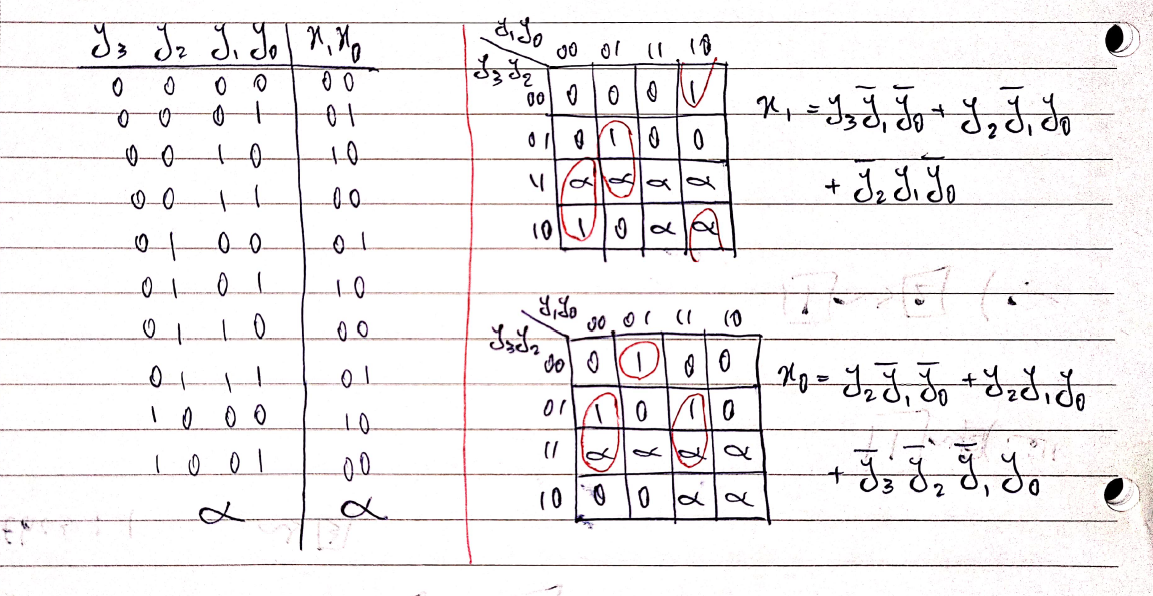
\includegraphics[width=0.8\linewidth]{karno}
\end{figure}
سپس ماژول دیگری به نام
$bcd\_3\_checker$
داریم که یک عدد 4رقمی $BCD$ را می‌گیرد و باقی مانده تمام ارقام آن عدد بر سه را با یکدیگر جمع می‌کند. مشخص است که این عدد حداکثر می‌تواند 8 باشد بنابراین با استفاده از همان ماژول اولیه، باقی ماتده این عدد را هم بر 3 می‌یابیم که درواقع برابر باقی مانده عدد بر 3 است. در پایان به کمک یک $or$ و $not$ بررسی می‌کنیم که اگر هر دو رقم باقی مانده برابر 0 بود خروجی 1 (به معنای بخش‌پذیری) و در غیر این صورت خروجی 0 شود.\\
برای بررسی بخش‌پذیری بر 11 از قاعده زیر استفاده شده است:
\begin{equation*}
\overline{abcd}\;mod\;11\,=\, (b\,+d\,-\,a\,-\,c)\; mod\;11
\end{equation*}
باتوجه به محدوده اعداد به سادگی می‌توان فهمید که اگر
$(b\,+d\,-\,a\,-\,c)\,=\,-11\,\vee \,0\,\vee \,11$
باشد عدد بر 11 بخش پذیر است و در غیر این صورت بخش‌پدیر نیست. به جای تفریق کردن ما مقادیر
$x\,=\,b\,+\,d$
و
$y\,=\,a\,+\,c$
را محاسبه می‌کنیم (به کمک یک $FullAdder$) و سپس به کمک یک مقایسه‌گر ( که در ماژول $five\_bit\_comprator$ نوشته شده است) ابتدا $x$ و $y$ و سپس $x$ و $y\,+\,11$ و سپس
$x\,+\,11$
و
$y$
را مقایسه می‌کنیم و در صورتی که حتی یکی از این مقایسه‌گرها اعلام برابری کند می‌گوییم که عدد بر 11 بخش‌پذیر است. (همچنین دقت کنید که مقایسه‌گر صرفا می‌گوید که آیا اعداد ورودی برابر هستند یا خیر)\\
گزارش برنامه برای تعداد $LUT$ به شکل زیر است:
\begin{center}
\begin{latin}
Slice Logic Utilization: \\
 Number of Slice LUTs:                   38  out of  63400     0\%  \\
    Number used as Logic:                38  out of  63400     0\%\\
\end{latin}
\end{center}
نتایج برنامه برای شبیه‌سازی در زیر آمده است (عکس‌ها در صورت نیاز برای بررسی بیشتر پیوست شده‌اند) :\\
\begin{figure}[H]
 \centering
  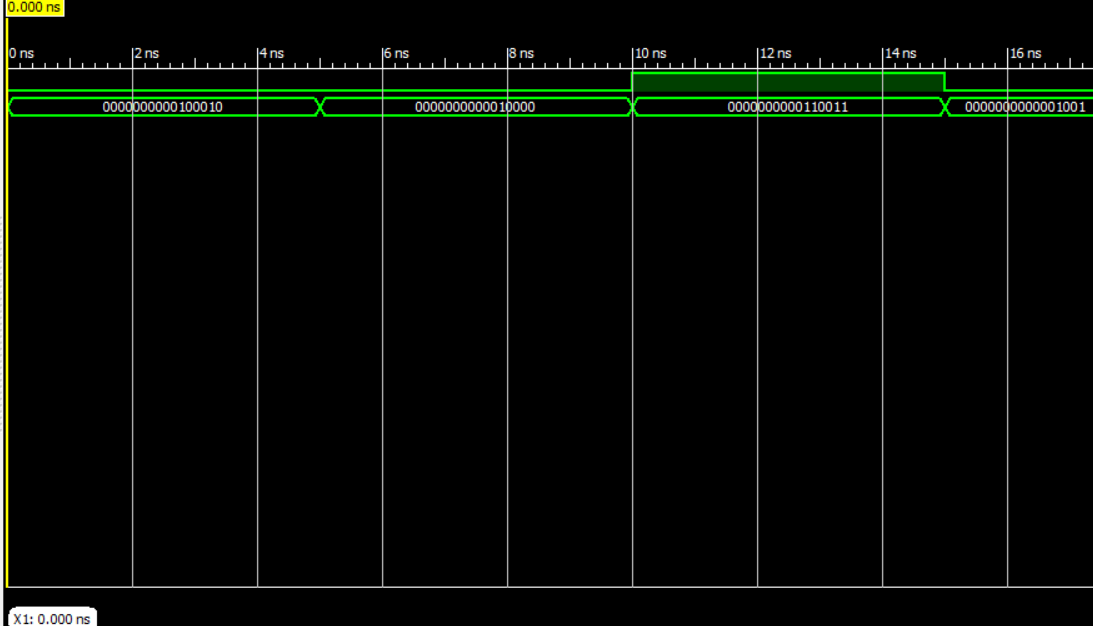
\includegraphics[width=0.8\linewidth]{s1}
\end{figure}
\begin{figure}[H]
 \centering
  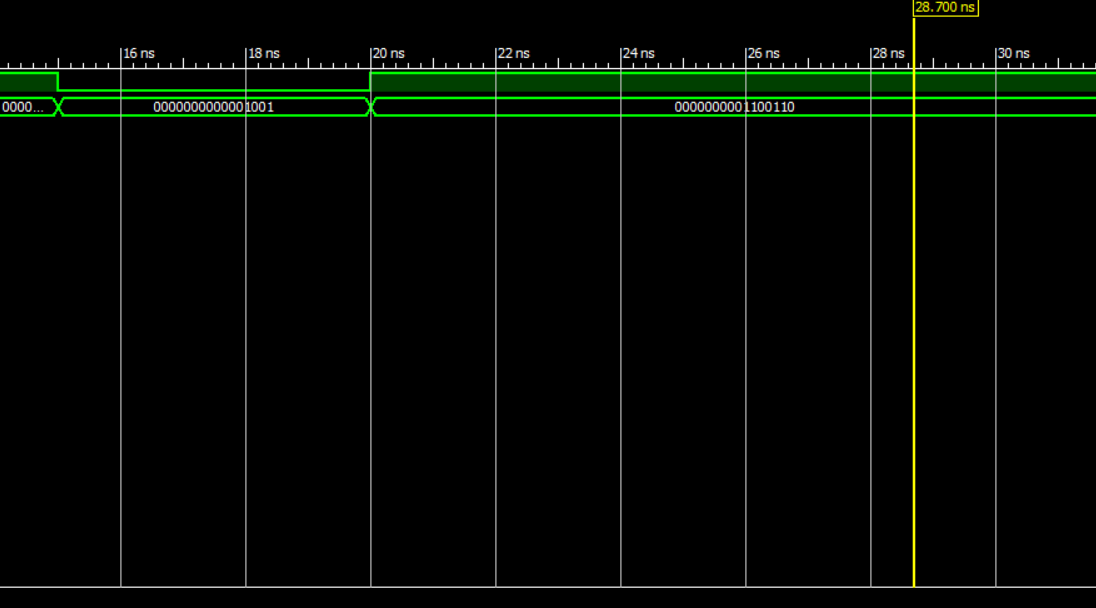
\includegraphics[width=0.8\linewidth]{s2}
\end{figure}
فایل کد اصلی در فایل
$checker.v$
قرار دارد و تست بنچ فایل ماژول در
$checker\_tb.v$
قرار دارد. تمامی تست بنچ‌ها در فایل
$checker\_tb\_all.v$
قرار دارند.\\
\pagebreak
در ادامه نیز شکل مدار قرار دارد، به علت شلوغی کد برای نمایش شکل از بلوک‌‌‌بندی استفاده کرده‌ایم:\\
ماژول $checker$:
\begin{figure}[H]
 \centering
  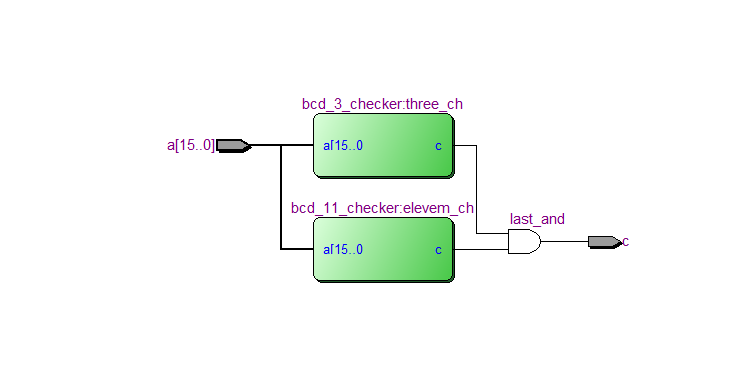
\includegraphics[width=0.8\linewidth]{sh1}
\end{figure}
ماژول
$bcd\_3\_checker$:
\begin{figure}[H]
 \centering
  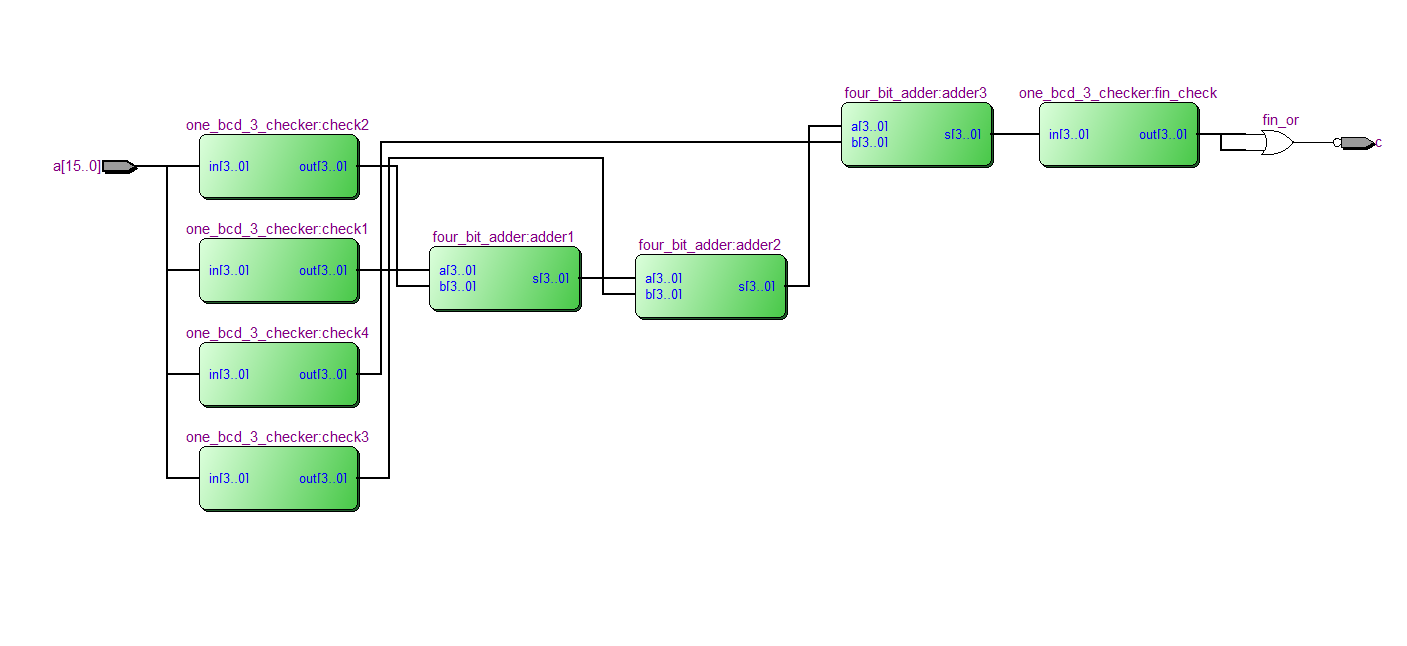
\includegraphics[width=0.8\linewidth]{sh2}
\end{figure}
ماژول
$one\_bcd\_3\_checker$:
\begin{figure}[H]
 \centering
  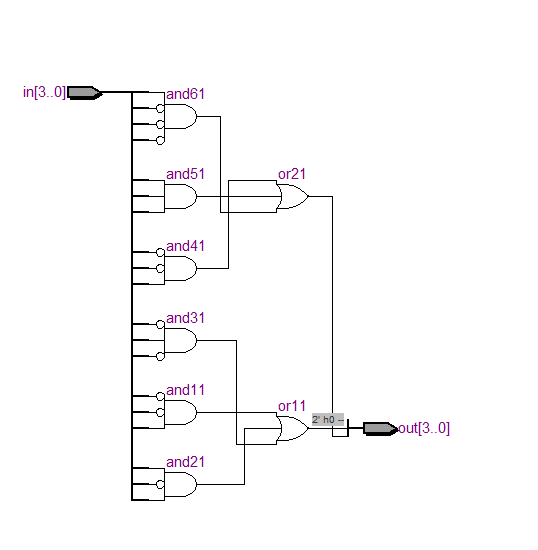
\includegraphics[width=0.8\linewidth]{sh3}
\end{figure}
ماژول
$bcd\_11\_checker$:
\begin{figure}[H]
 \centering
  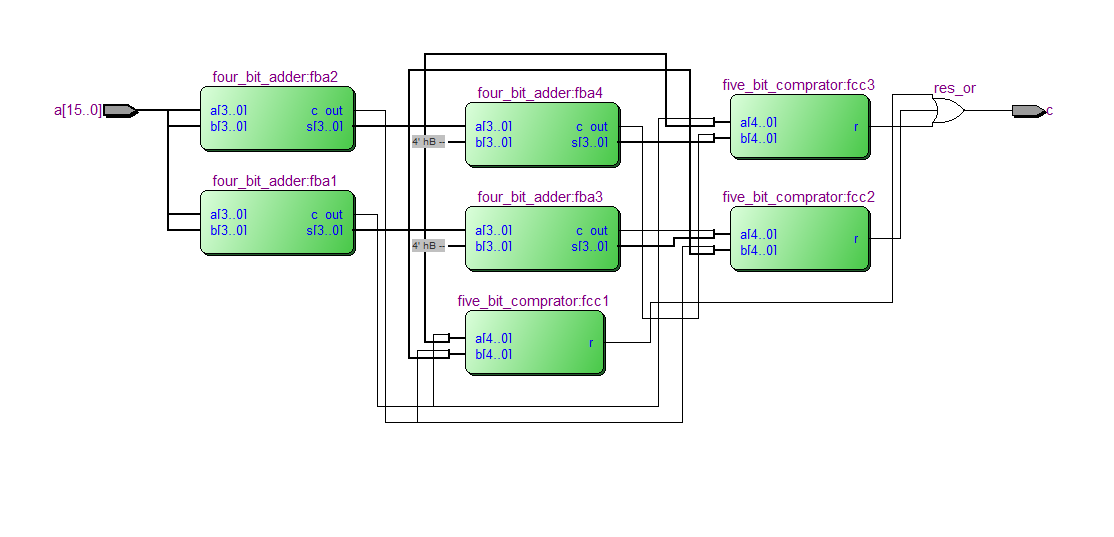
\includegraphics[width=0.8\linewidth]{sh4}
\end{figure}
ماژول
$four\_bit\_adder$:
\begin{figure}[H]
 \centering
  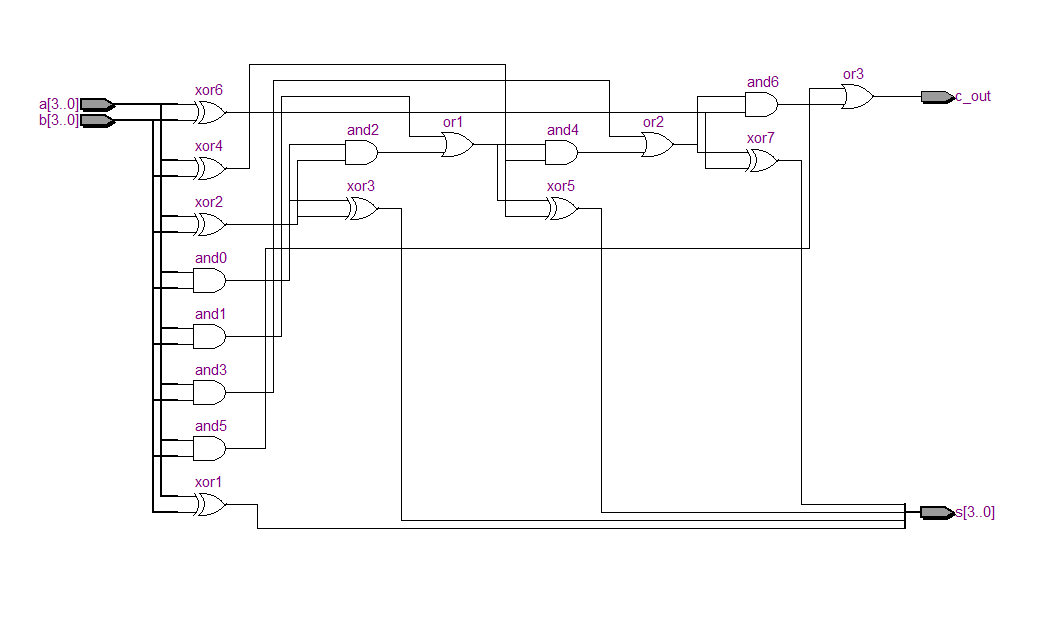
\includegraphics[width=0.8\linewidth]{sh5}
\end{figure}
ماژول
$five\_bit\_comprator$:
\begin{figure}[H]
 \centering
  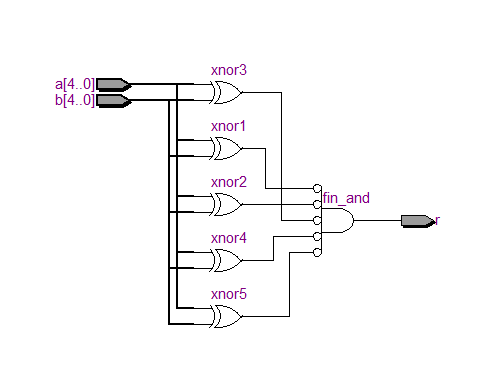
\includegraphics[width=0.8\linewidth]{sh6}
\end{figure}
\end{document}